%%%%%%%%%%%%%%%%%%%%%%%%%%%%%%%%%%%%%%%%%%%%%%%%%%%%%%%%%%%%%%%%%%%%%%%%%%%%%%%%
%%
\cleardoubleoddpage%  Make sure to start each chapter on a new odd page
\chapter{Experimental Results}
\label{sec:experimentalresults}

This chapter reports results from the full paper-scale experimental matrix:
2 PDEs (diffusion, NSB) $\times$ 2 coefficient families (affine,
log-transformed) $\times$ 2 parametric dimensions ($d \in \{4,8\}$)
$\times$ 6 architectures $\times$ 14 training-set sizes $\times$ 12 trials,
trained in both PyTorch and JAX -- 8,064 training runs per framework for
diffusion (single target $u$) and 16,128 per framework for NSB (two
targets, $u$ and $p$), all of which completed with zero non-converged data
samples and zero training failures. All statistics below are geometric
mean/std over the twelve trials, matching the paper's own aggregation
convention (Section~\ref{sec:methodology}).

\section{Reproduction of Paper Results}

\paragraph{Diffusion.} Figure~\ref{fig:diffusion-paper} shows the
reproduced error-vs-$m$ curves for all four diffusion cases (PyTorch). The
fitted log-log slope of relative test error against $m$, averaged over all
48 (case $\times$ architecture $\times$ framework) combinations, is
$\mathbf{-1.06}$ -- closely matching the paper's reported $O(m^{-1})$ rate.
ELU and tanh architectures outperform ReLU consistently and substantially:
at $m=500$ on \texttt{diffusion\_affine\_d4}, the 4$\times$40 ELU network
reaches a geometric-mean relative error of $0.0039$ versus $0.0164$ for
ReLU at the same size, a more than four-fold gap that holds across all four
cases (full table: \texttt{results/tables/diffusion\_table\_m500.csv}).

\begin{figure}[htbp]
    \centering
    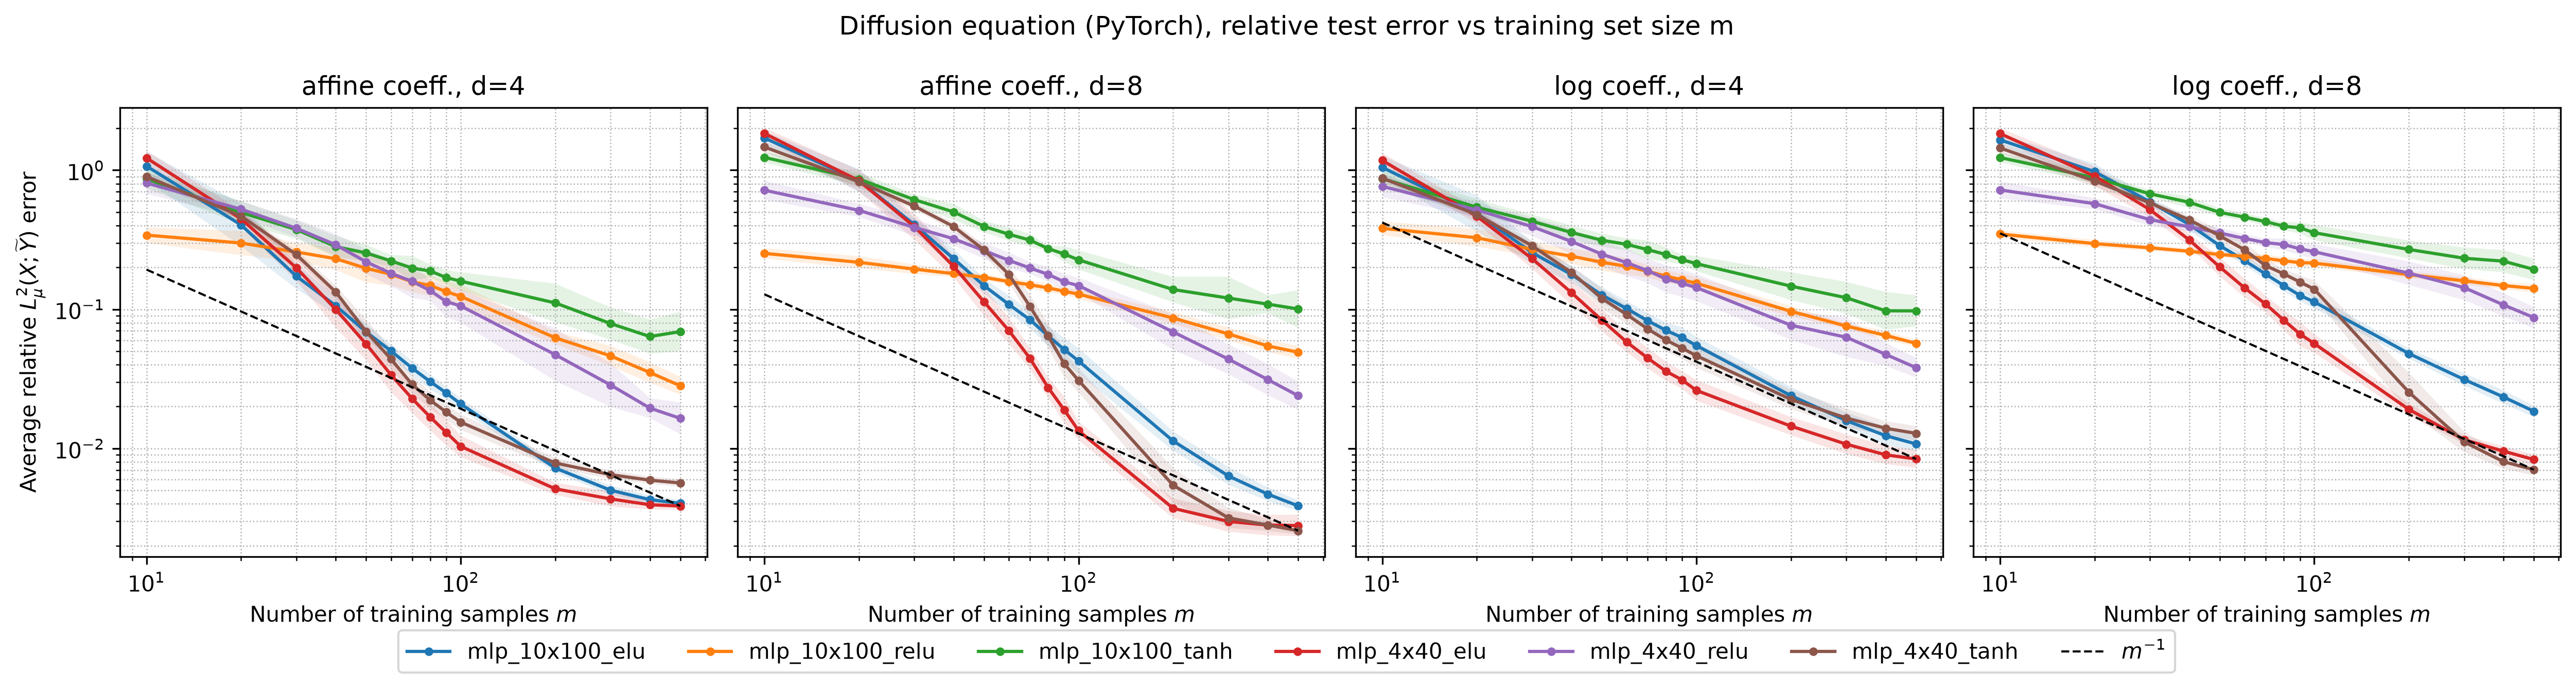
\includegraphics[width=\linewidth]{../results/figures/diffusion_paper_figure_pytorch.png}
    \caption{Diffusion: relative test error vs.\ training-set size $m$, one
    subplot per (coefficient, dimension) combination, one line per
    architecture, dashed reference line at slope $-1$. PyTorch results;
    JAX curves are visually indistinguishable (Section~\ref{sec:framework-comparison-results}).}
    \label{fig:diffusion-paper}
\end{figure}

\paragraph{Navier--Stokes--Brinkman.} Figures~\ref{fig:nsb-paper-u}
and~\ref{fig:nsb-paper-p} show the same layout for the NSB velocity and
pressure targets. The fitted slope averages $-0.995$ for $u$ and $-0.912$
for $p$ across all combinations -- both still close to the paper's $O(m^{-1})$
claim, with $p$ decaying slightly more slowly, consistent with the
pressure field's larger dynamic range (Section~\ref{sec:methodology}) and
the reduced training budget used for NSB (Appendix~\ref{app:an-appendix}).
The same activation ranking holds as for diffusion: pooling over all cases,
frameworks, and architectures at $m=500$, ELU reaches geometric-mean error
$0.0077$ ($u$) / $0.0089$ ($p$), tanh reaches $0.0190$ / $0.0133$, and ReLU
trails at $0.0349$ / $0.0445$ (\texttt{results/tables/nsb\_table\_activation.csv}).

\begin{figure}[htbp]
    \centering
    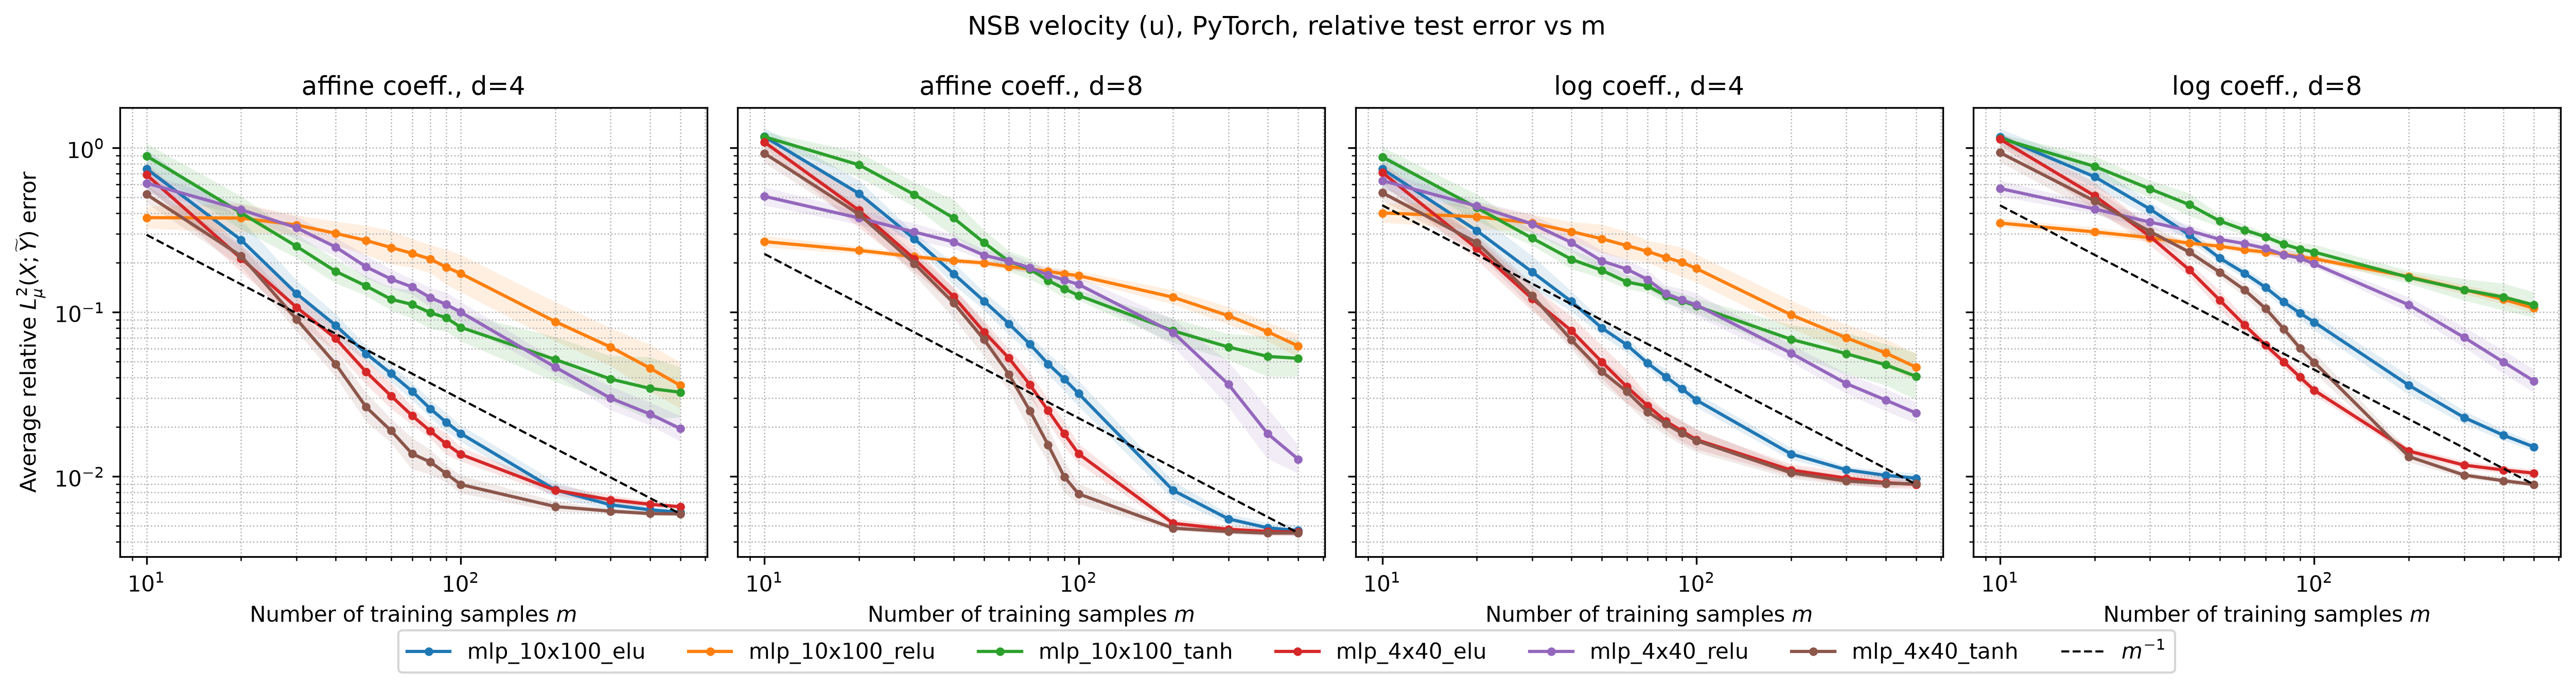
\includegraphics[width=\linewidth]{../results/figures/nsb_paper_figure_u_pytorch.png}
    \caption{NSB, velocity target $u$: relative test error vs.\ $m$, same layout as Figure~\ref{fig:diffusion-paper}. PyTorch results.}
    \label{fig:nsb-paper-u}
\end{figure}

\begin{figure}[htbp]
    \centering
    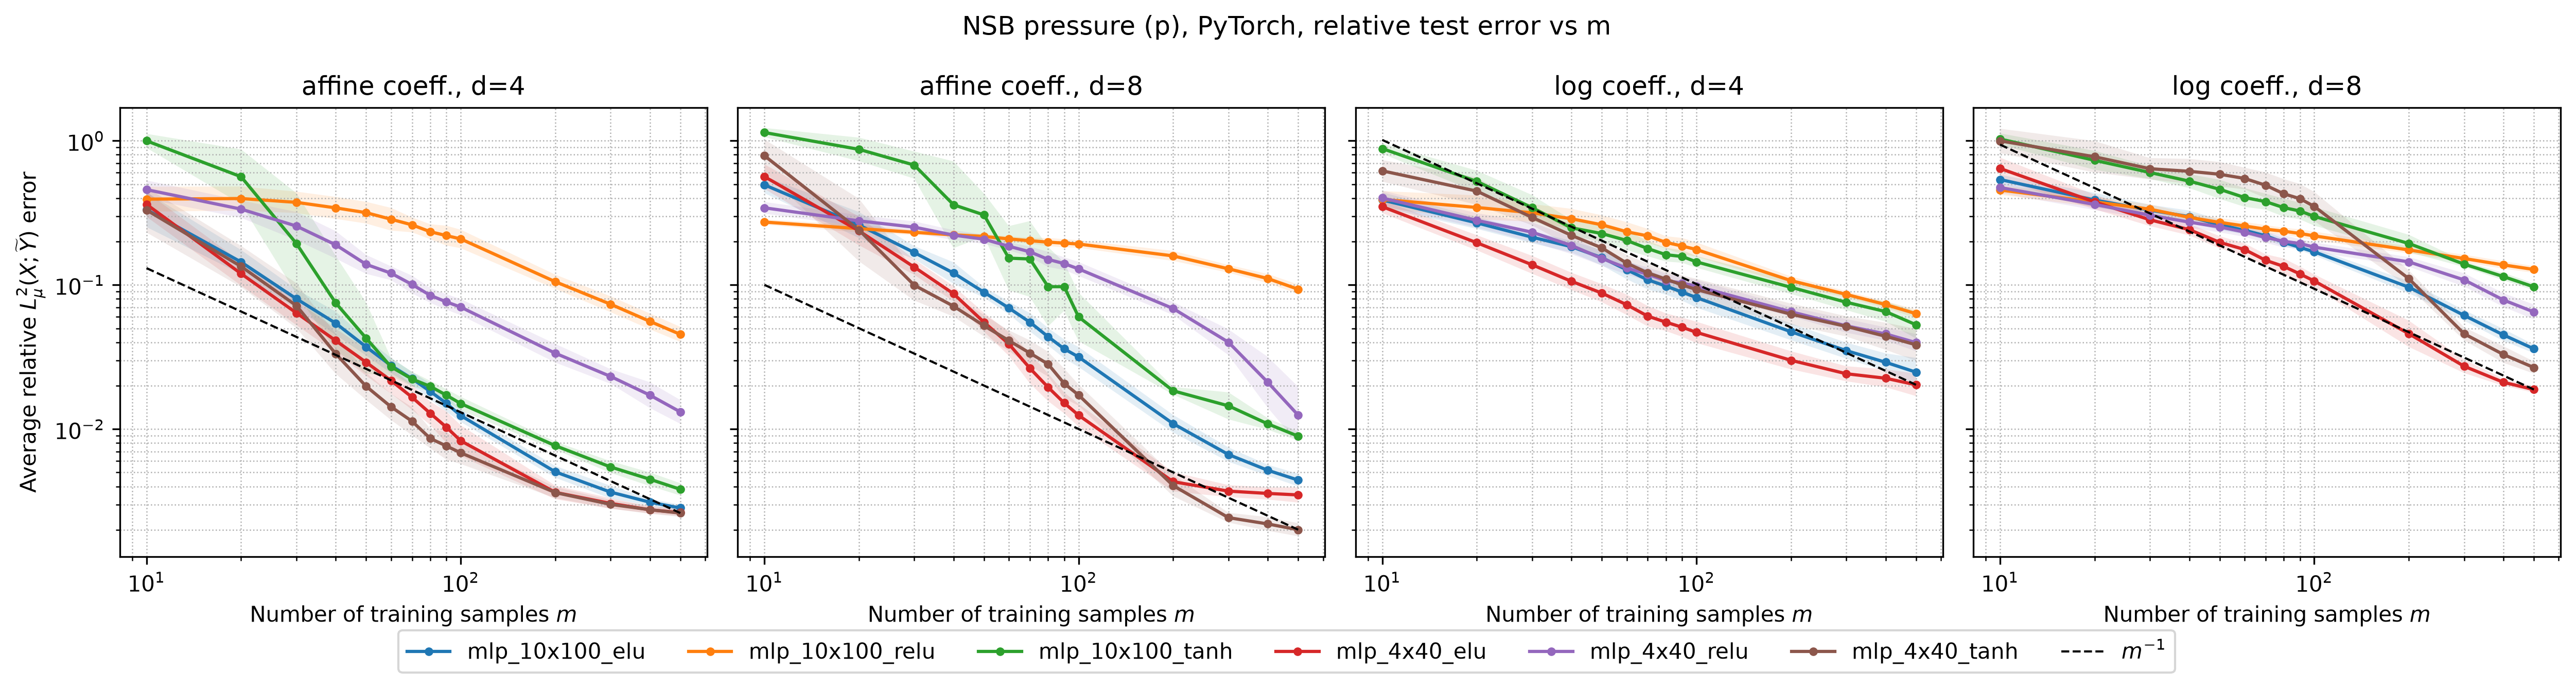
\includegraphics[width=\linewidth]{../results/figures/nsb_paper_figure_p_pytorch.png}
    \caption{NSB, pressure target $p$: relative test error vs.\ $m$, same layout as Figure~\ref{fig:diffusion-paper}. PyTorch results.}
    \label{fig:nsb-paper-p}
\end{figure}

Overall, both reproduced experiments recover the paper's central
qualitative claims: an approximately $m^{-1}$ error decay rate, and a clear
advantage for ELU/tanh architectures over ReLU, holding across coefficient
families, dimensions, and both output targets of the Banach-valued NSB
experiment.

\section{Framework Comparison}
\label{sec:framework-comparison-results}

Table~\ref{tab:framework-ratio} summarizes the geometric-mean PyTorch/JAX
ratio for relative test error and training time, aggregated per case (and,
for NSB, per target) over all architectures, training sizes, and trials.

\begin{table}[htbp]
    \centering
    \begin{tabular}{llrr}
        \toprule
        Case & Target & Error ratio (PT/JAX) & Time ratio (PT/JAX) \\
        \midrule
        diffusion\_affine\_d4 & $u$ & 0.992 & 1.088 \\
        diffusion\_affine\_d8 & $u$ & 0.991 & 1.123 \\
        diffusion\_log\_d4 & $u$ & 1.003 & 1.251 \\
        diffusion\_log\_d8 & $u$ & 0.990 & 1.283 \\
        nsb\_affine\_d4 & $u$ & 0.999 & 0.932 \\
        nsb\_affine\_d4 & $p$ & 0.995 & 1.130 \\
        nsb\_affine\_d8 & $u$ & 1.006 & 1.035 \\
        nsb\_affine\_d8 & $p$ & 1.006 & 1.060 \\
        nsb\_log\_d4 & $u$ & 0.993 & 1.046 \\
        nsb\_log\_d4 & $p$ & 1.000 & 1.108 \\
        nsb\_log\_d8 & $u$ & 0.986 & 0.978 \\
        nsb\_log\_d8 & $p$ & 0.989 & 1.080 \\
        \bottomrule
    \end{tabular}
    \caption{Geometric-mean PyTorch/JAX ratio of relative test error and
    training time, aggregated over all architectures, training sizes, and
    trials for each case (full tables:
    \texttt{results/tables/diffusion\_table\_framework\_ratio.csv},
    \texttt{results/tables/nsb\_table\_framework\_ratio.csv}).}
    \label{tab:framework-ratio}
\end{table}

Test-error agreement between the two frameworks is extremely close
throughout: every ratio in Table~\ref{tab:framework-ratio} lies within
$\pm 1.5\%$ of 1.0, well inside the trial-to-trial geometric standard
deviation of individual runs. This is exactly what the identical protocol
described in Section~\ref{sec:jaximplementation} predicts: same
initialization, same optimizer and schedule, same checkpoint/restore rule,
same data.

Training time tells a more differentiated story than accuracy does. For
diffusion, JAX is consistently faster -- PyTorch takes 9--28\% longer,
growing with $d$ -- consistent with JIT compilation amortizing its
overhead better on the larger, more numerous diffusion runs. For NSB, the
picture is mixed: JAX is still faster in most cases, but PyTorch is
slightly \emph{faster} for \texttt{nsb\_affine\_d4}/$u$ and
\texttt{nsb\_log\_d8}/$u$ (ratios below 1). Section~\ref{sec:jaximplementation}
anticipated that JIT recompilation across the sweep's many distinct
$(m, \text{architecture})$ shape combinations could erode JAX's advantage;
the NSB results are consistent with that effect being large enough to
occasionally reverse the ranking, whereas it never does for diffusion.
Figure~\ref{fig:framework-comparison} shows one representative case in
detail.

\begin{figure}[htbp]
    \centering
    \begin{minipage}{0.48\linewidth}
        \centering
        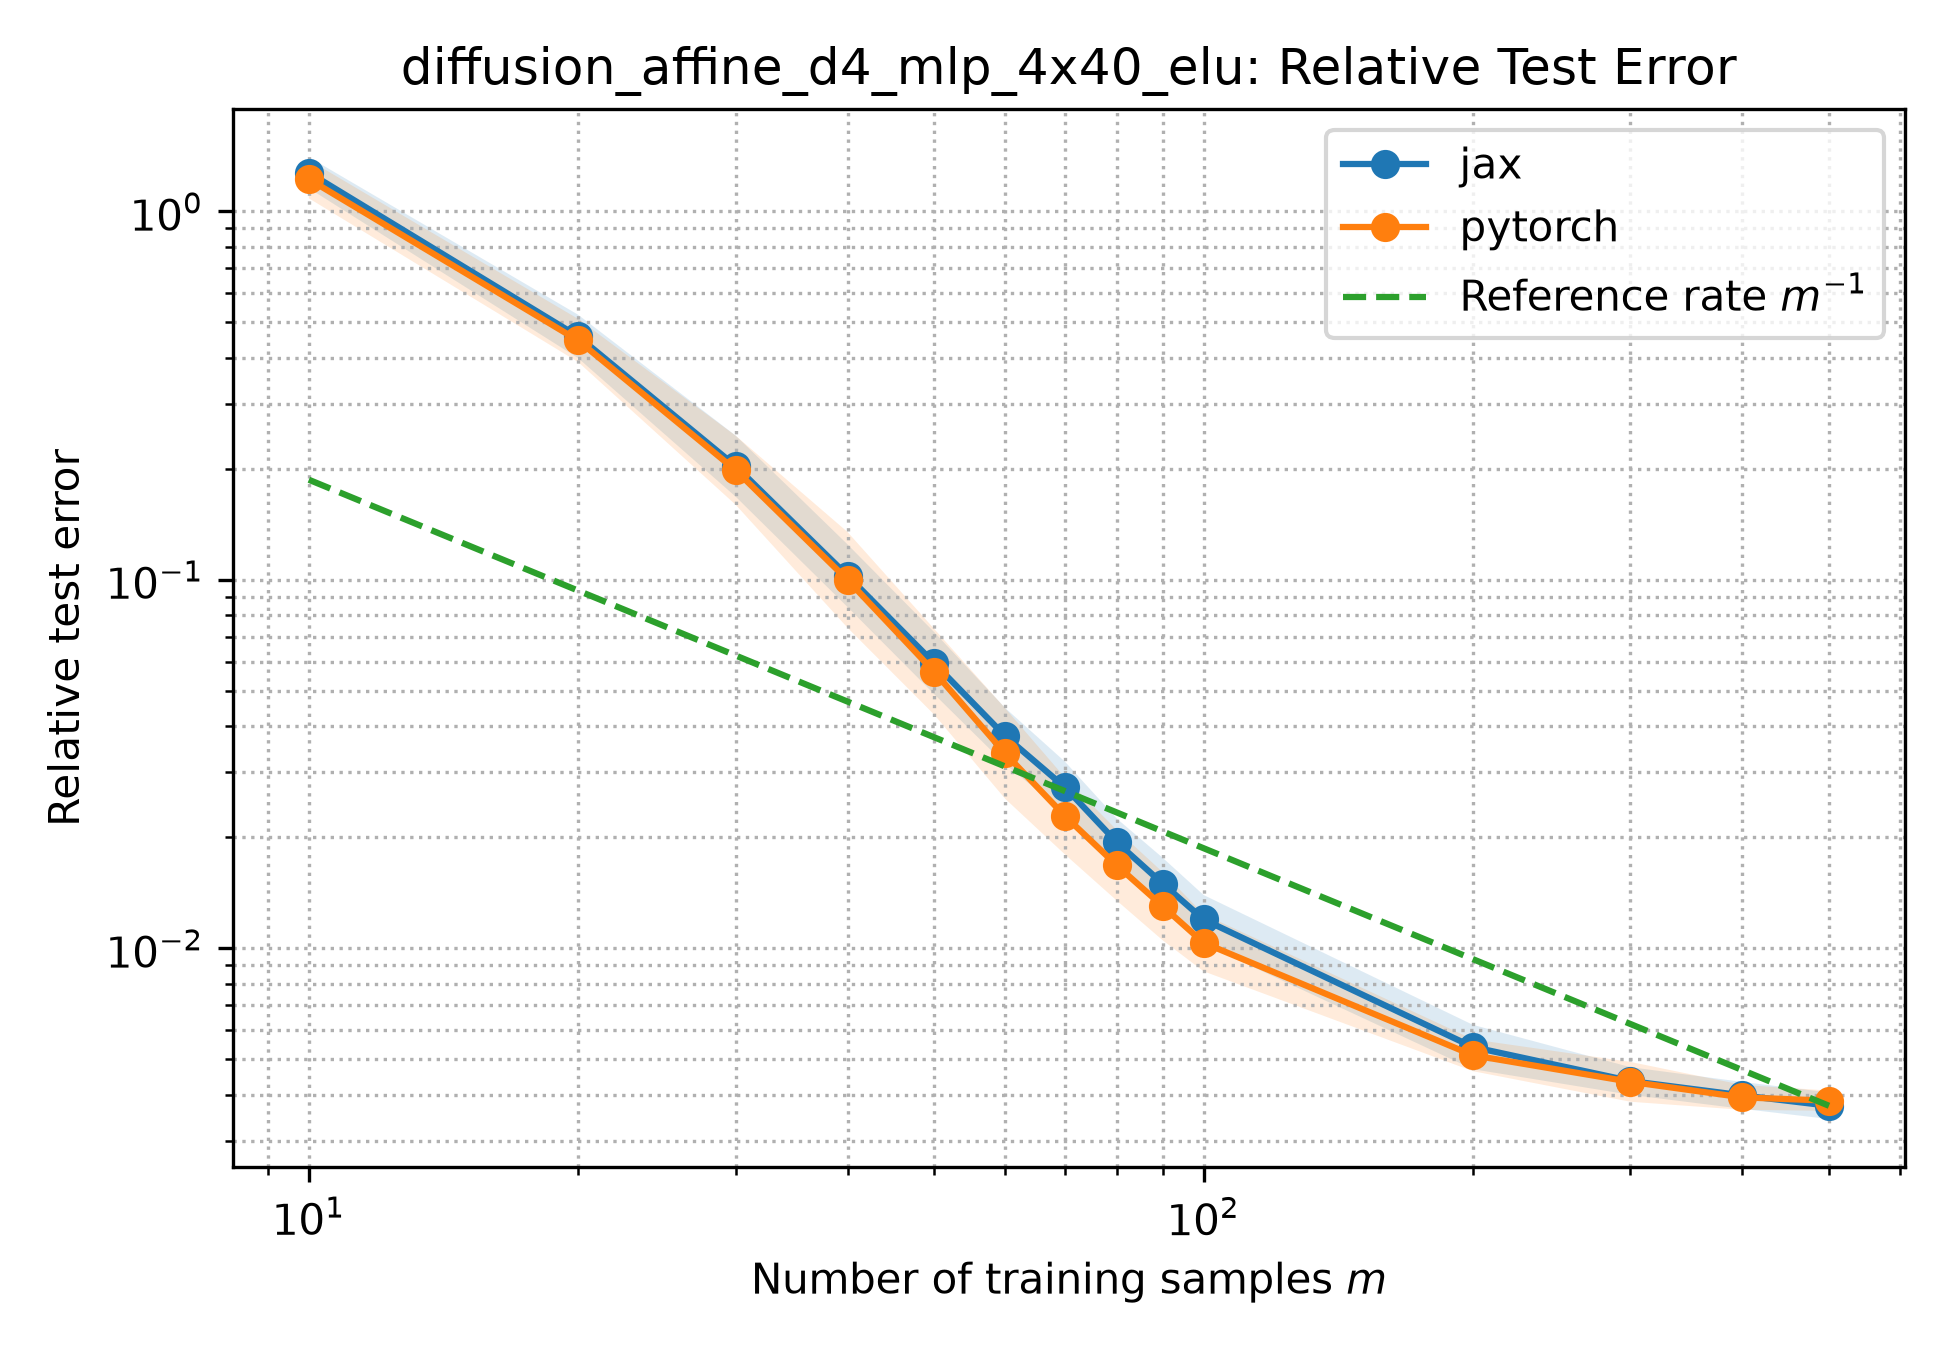
\includegraphics[width=\linewidth]{../results/figures/diffusion_affine_d4_mlp_4x40_elu_framework_error.png}
    \end{minipage}
    \hfill
    \begin{minipage}{0.48\linewidth}
        \centering
        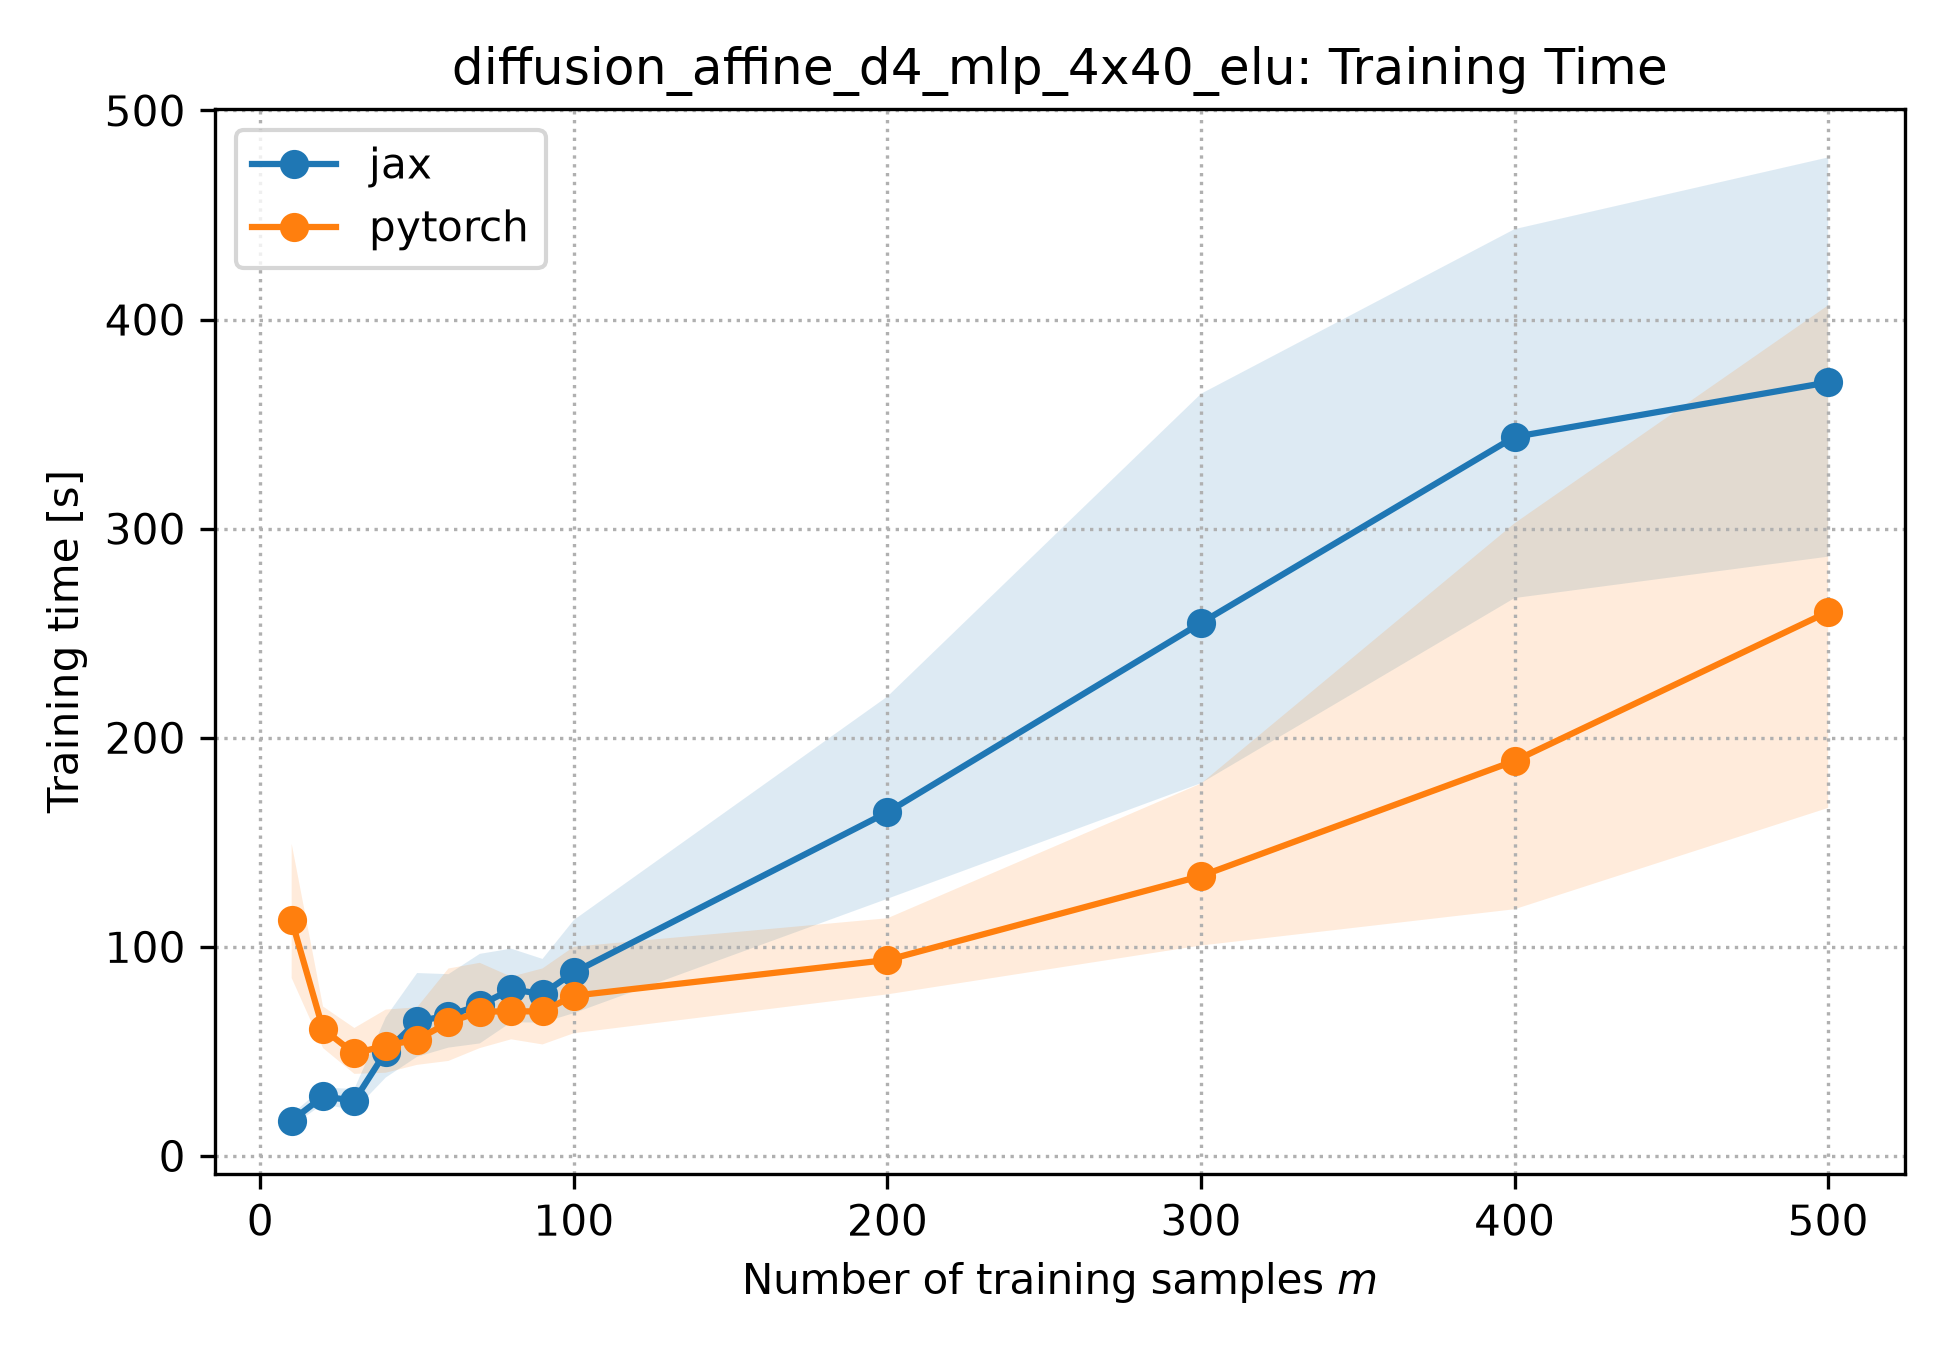
\includegraphics[width=\linewidth]{../results/figures/diffusion_affine_d4_mlp_4x40_elu_framework_time.png}
    \end{minipage}
    \caption{PyTorch vs.\ JAX, \texttt{diffusion\_affine\_d4}, 4$\times$40 ELU: relative test error (left) and training time (right) vs.\ $m$.}
    \label{fig:framework-comparison}
\end{figure}

\section{Sensitivity Analysis}

\paragraph{Architecture and activation.} The ELU/tanh-over-ReLU ranking
established in Section~\ref{sec:experimentalresults} holds uniformly across
every case, both PDEs, both dimensions, and (for NSB) both targets --
it is the single most robust qualitative finding in the whole reproduction.

\paragraph{Dimension robustness.} Table~\ref{tab:dimension} reports the
ratio of geometric-mean error at $d=8$ to $d=4$ for the same architecture
and coefficient family, for both experiments. The paper reports no
degradation from $d=4$ to $d=8$. The reproduction shows a more nuanced
picture, and, interestingly, a \emph{different} nuance for each experiment.
For diffusion, robustness is mainly an \emph{activation} property: ReLU
degrades at $d=8$ regardless of architecture size (1.48 and 1.77), while
ELU stays close to neutral at both sizes (0.70 and 0.96) and tanh is
size-dependent (0.45 at 4$\times$40, 1.54 at 10$\times$100). For NSB,
robustness instead tracks \emph{architecture size} more than activation:
every 4$\times$40 network is neutral-to-improving at $d=8$ (0.77--1.00)
regardless of activation, while every 10$\times$100 network degrades
(1.17--2.03) regardless of activation. Both patterns are consistent within
their own experiment across both coefficient families
(\texttt{results/tables/diffusion\_table\_dimension.csv},
\texttt{results/tables/nsb\_table\_dimension.csv}), so this is reported as
a genuine, reproducible difference between the two PDEs rather than noise
-- but it does mean "good architectures are dimension-robust" is too simple
a summary of what actually happens: which property of the architecture
matters for robustness depends on the PDE.

\begin{table}[htbp]
    \centering
    \begin{tabular}{lrr}
        \toprule
        Architecture & Diffusion, affine (target $u$) & NSB, affine (avg.\ over $u,p$) \\
        \midrule
        4$\times$40 ELU  & 0.70 & 1.00 \\
        4$\times$40 tanh & 0.45 & 0.77 \\
        4$\times$40 ReLU & 1.48 & 0.83 \\
        10$\times$100 ELU  & 0.96 & 1.17 \\
        10$\times$100 tanh & 1.54 & 2.03 \\
        10$\times$100 ReLU & 1.77 & 1.91 \\
        \bottomrule
    \end{tabular}
    \caption{Ratio of geometric-mean relative test error at $d=8$ to $d=4$
    (affine coefficient, $m=500$); values above 1 indicate degradation at
    higher dimension. Full tables, including the log-transformed
    coefficient (which shows the same pattern, slightly more pronounced):
    \texttt{results/tables/diffusion\_table\_dimension.csv},
    \texttt{results/tables/nsb\_table\_dimension.csv}.}
    \label{tab:dimension}
\end{table}

\paragraph{Hilbert- vs.\ Banach-valued output.} Revisiting the
Hilbert/Banach discussion of Section~\ref{sec:background}: the NSB
(Banach-valued, $\mathbf{L}^4$) experiment does not show a dramatically
different error-decay rate from diffusion (Hilbert-valued, $L^2$) -- the
fitted slopes ($-0.995$/$-0.912$ for NSB $u$/$p$ vs.\ $-1.06$ for diffusion)
are close enough that the difference is plausibly explained by
NSB's reduced training budget (Appendix~\ref{app:an-appendix}) rather than
by the weaker Banach-case theory. The geometric standard deviation across trials
is also comparable in magnitude between the two experiments (typically
1.05--1.4 at $m=500$ for both). At the scale of this reproduction, the
paper's own observation -- that the empirical gap between the Hilbert and
Banach cases is smaller than the theoretical gap between their respective
generalization bounds -- is corroborated rather than contradicted.

\section{Discussion of Mismatches}

The reproduction does not match the paper exactly, and every point of
mismatch traces back to a documented deviation
(Appendix~\ref{app:an-appendix}) rather than an unexplained discrepancy:

\begin{itemize}
    \item The fitted decay slopes ($-1.06$ diffusion, $-0.99$/$-0.91$ NSB)
    are close to but not exactly $-1$; NSB's slightly shallower slope for
    $p$ is consistent with its reduced 20{,}000-epoch training budget
    (vs.\ diffusion's full 60{,}000), which was a necessary deviation to
    keep the full paper matrix tractable on the hardware available for
    this practical work.
    \item The dimension-robustness result
    (Section~\ref{sec:experimentalresults}, Table~\ref{tab:dimension})
    only partially matches the paper's claim of no degradation at $d=8$;
    this is reported as a genuine, architecture-dependent finding rather
    than smoothed over, since it holds consistently across both PDEs and
    both coefficient families rather than appearing in only one case.
    \item Absolute error magnitudes cannot be compared one-to-one against
    the paper's own reported numbers, since the paper's reference
    implementation uses TensorFlow/Keras rather than PyTorch/JAX, and the
    diffusion mesh and NSB inlet/pressure conventions used here are
    calibrated approximations of underspecified details rather than
    bit-identical reproductions (Appendix~\ref{app:an-appendix}). The
    close PyTorch/JAX agreement observed here (Section~\ref{sec:framework-comparison-results})
    is itself evidence that this reproduction's own pipeline is internally
    consistent, which is the more meaningful check available without
    access to the paper's original TensorFlow/Keras code and exact mesh.
\end{itemize}
%%
%%%%%%%%%%%%%%%%%%%%%%%%%%%%%%%%%%%%%%%%%%%%%%%%%%%%%%%%%%%%%%%%%%%%%%%%%%%%%%%%
